\chapter{Introduction}
\label{chap:Chapter1}

\glspl{uav} have witnessed a surge in popularity and research attention.
They have become indispensable in various applications, ranging from surveillance to reconnaissance, due to their versatility and efficiency in various applications \cite{UAV1}.

This growing interest is evident in the numerous review papers exploring different aspects of \gls{uav} development, ranging from open-source hardware and software utilization \cite{UAV2}, frame design and optimization \cite{UAV5}, control systems, including both conventional and modern communication modalities such as 5G networks \cite{UAV7}, to efficient power management strategies, and alternative energy sources to extend \gls{uav} battery life \cite{UAV12}. %, \cite{UAV3},\cite{UAV4} || \cite{UAV6} || , \cite{UAV8}, \cite{UAV10}, \cite{UAV11}

Nowadays, most \gls{VTOL} \glspl{uav}, rely on proprotors with fixed pitch systems because of their simplicity and lack of better \gls{COTS} reliable and efficient solutions but they impose limitations on the achievable flight performance \cite{FPP1}.
Thrust generation is confined to a single direction, hindering the \gls{uav}'s ability to produce upward thrust relative to the vehicle body.
Additionally, the \glspl{uav} control is restricted by the inertia of the motors and proprotors, constraining the \gls{uav}'s agility and maneuverability \cite{FPP1}.
As described in recent studies \cite{FPP1}, these limitations become more pronounced as \gls{uav} size increases, impacting stability and control.
Larger \glspl{uav} face challenges as the need for larger motors with higher inertia compromises rapid control through \gls{RPM} adjustments alone.

The development of Variable Pitch Proprotor (VPP) systems plays a crucial role in overcoming the limitations of traditional \gls{uav} designs, such as those with fixed pitch proprotors \cite{FPP1}, \cite{VPP1}.
Several detailed descriptions of quadrotors, for instance, modeling and dynamics have been published \cite{FPP2}, \cite{FPP3}, \cite{FPP4}, \cite{FPP5}, emphasizing the need for dynamic control mechanisms.
The use of VPP systems, especially in \gls{VTOL} \glspl{uav}, addresses challenges related to control instabilities and energy efficiency \cite{VPP1}.

The incorporation of variable-pitch proprotors provides the necessary flexibility to enhance stability and enable larger \glspl{uav} to perform sophisticated maneuvers, overcoming the constraints inherent in fixed-pitch designs \cite{FPP1}, \cite{VPP1}.
The graphs shown in figure \ref{fig:FPPvsVPP2} and \ref{fig:FPPvsVPP}, illustrate the differences between fixed-pitch and variable-pitch propellers (constant-speed in this graphs).

\begin{figure}[H]
    \centering
    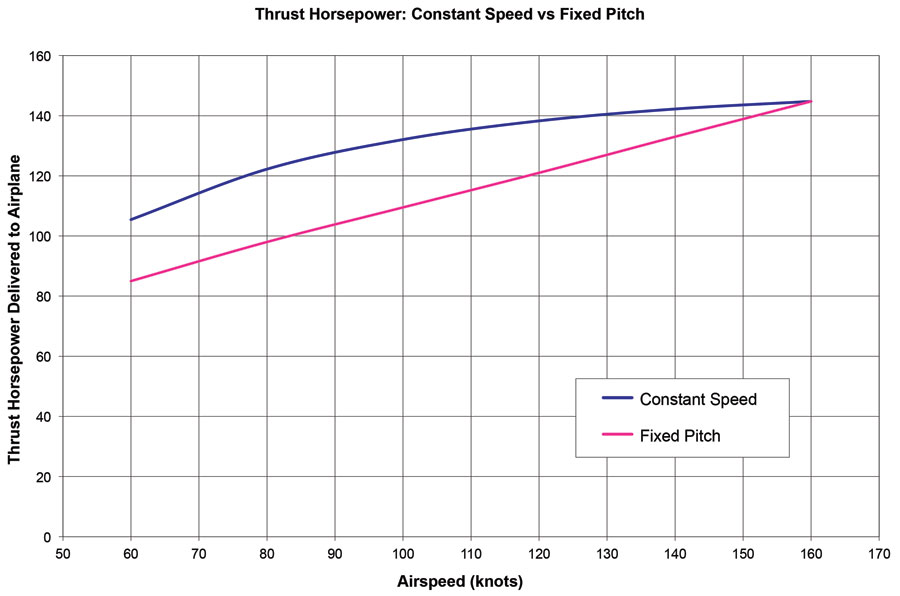
\includegraphics[scale=0.45]{ch1/assests/FPPvsVPP2.jpg}
    \caption{\cite{VPP7}}
    \label{fig:FPPvsVPP2}
\end{figure}

\begin{figure}[H]
    \centering
    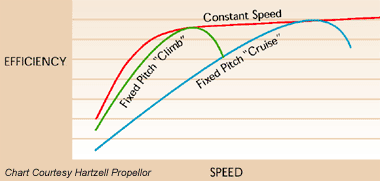
\includegraphics[scale=0.8]{ch1/assests/FPPvsVPP.png}
    \caption{\cite{VPP9}}
    \label{fig:FPPvsVPP}
\end{figure}

It is possible to see that when the propeller reaches its maximum airspeed design point, there is little to no difference between the performance of the fixed-pitch and variable-pitch propellers.
The difference in performance and efficiency can be seen when the airspeed is below or above the maximum design point \cite{VPP9}.

This Thesis aims to develop a stand-alone variable-pitch proprotor system that can, in real-time, change the propeller pitch according to each flight phase.
This work will be integrated into a PhD Thesis that is currently being developed at Universidade da Beira Interior by Eng. Renato Machado about Urban Air Mobility.

%-------------------------------------------------------------------------------%

\section{Problem Analysis}
The utilization of fixed-pitch propellers in \glspl{uav} presents a set of limitations that significantly impact aircraft performance and efficiency.
These issues are evident in various phases of flight, including hover and forward flight, and have repercussions for the \gls{uav}.

In terms of maneuverability and response, fixed-pitch propellers inherently constrain the \glspl{uav} from adjusting the pitch angle during flight \cite{FPP1}.
This limitation results in compromised maneuverability and response, restricting the range of aerobatic maneuvers that a \gls{uav} can execute \cite{FPP1}.
Additionally, the inability to change the pitch angle impedes the optimization of lift, landing, and thrust during flight, leading to sub-optimal performance in various operational scenarios \cite{FPP1}.

As for power consumption in systems with fixed-pitch propellers, the power consumption will be higher.
Without the ability to adjust the propeller angle, the \glspl{uav} may be forced to operate at higher \glspl{RPM} to compensate for this lack of adjustment \cite{FPP1}.
This higher power consumption not only affects the efficiency of the \gls{uav} but also has implications for its endurance, limiting the time the vehicle can remain airborne.


%-------------------------------------------------------------------------------%

\section{Motivation}
TODO: MORE INFO

%-------------------------------------------------------------------------------%

\section{Objectives}
As explained before, the focus will be on developing a stand-alone variable-pitch proprotor system.

The first goal will be the understanding of the relevant fundamentals regarding \gls{VTOL} flight performance and the impact of variable proprotors.

Next, describe the fundamentals of control subsystems, power management and short-range wireless communication protocols with particular emphasis on their reliability and real-time sensing and actuation.
There will also be made a survey about current solutions, communication technologies, electronic control and power management strategies.

After the research, it will be designed the subsystems architecture and then implemented the envisaged subsystem over a real mechanical prototype.

Finally, the performance of the system will be evaluated together with its limitations under different settings and environments.
